% !TEX root = exercises.tex

\exercisetitle{Exercise Sheet 1}

\begin{questions}
\question Use the triangle inequality $\abs{z_1-z_2} \leq \abs{z_1} + \abs{z_2}$ to prove the reverse triangle inequality:
\[
\abs{z_1-z_2} \geq \abs{\abs{z_1}-\abs{z_2}}
\]
\begin{answer}
The triangle inequality gives
\begin{align*}
\abs{z_1} & = \abs{z_1-z_2+z_2} \leq \abs{z_1-z_2} + \abs{z_2}  \\
\abs{z_2} & = \abs{z_2-z_1+z_1} \leq \abs{z_2-z_1} + \abs{z_1}\ (=\abs{z_1-z_2}+\abs{z_1}).
\end{align*}
Rearranging gives the two inequalities
\begin{align*}
\abs{z_1-z_2} & \geq \abs{z_1} - \abs{z_2} \\
\abs{z_1-z_2} & \geq \abs{z_2} - \abs{z_1},
\end{align*}
or in other words
\[
\abs{z_1-z_2} \geq \max \left( \abs{z_1}-\abs{z_2} , \abs{z_2} - \abs{z_1} \right) = \abs{\abs{z_1} - \abs{z_2} }.
\]
\end{answer}
\question Use the triangle and reverse triangle inequalities to show that for all $z$ on the circle $\abs{z}=2$, we have
\[
\abs{z+2} \leq 4 \text{ and } \abs{z-3+4i} \geq 3.
\]
Describe these inequalities geometrically.
\begin{answer}
If $\abs{z}=2$ then the triangle inequality ensures that
\[
\abs{z+2} \leq \abs{z}+2 = 4,
\]
and the backwards triangle inequality gives
\begin{align*}
\abs{z-3+4i} & = \abs{z-(3-4i)} \\
& \geq \abs{ \abs{z} - \abs{3-4i} } \\
& = \abs{2-5} = 3.
\end{align*}
Geometrically, these inequalities show respectively that the circle $\abs{z}=2$ is
\begin{itemize}
\item Contained in the disc with centre $-2$ and radius $4$ (i.e., the disc $\abs{z+2} \leq 4$), and
\item Outside of the disc with centre $3-4i$ and radius $3$.
\end{itemize}
\begin{center}
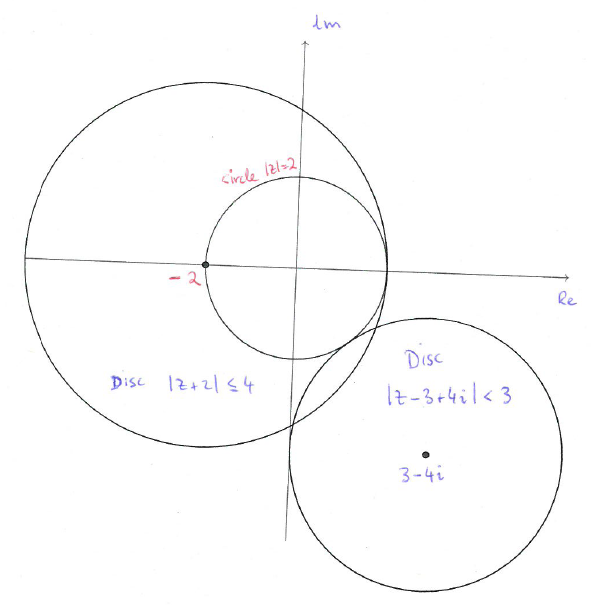
\includegraphics[scale=0.5]{ex1_q2}
\end{center}
\end{answer}
\question Use the triangle and reverse triangle inequalities to show that for all $z$ on the circle $\abs{z+3i}=3$ we have
\[
\abs{z-4} \leq 8,\quad \abs{z+5i}\geq 1 \text{ and } \abs{ \frac{z-4}{z+5i} } \leq 8.
\]
\begin{answer}

As with the previous question, the triangle inequality yields
\begin{align*}
\abs{z-4} & = \abs{z+3i-(3i+4)} \\
& \leq \abs{z+3i} + \abs{3i+4} \\
&=3+5=8.
\end{align*}
and the backwards triangle inequality yields
\begin{align*}
\abs{z+5i} & = \abs{z+3i+2i} \\
& \geq \abs{ \abs{z+3i} - \abs{2i} } \\
&=3-2=1.
\end{align*}
The third inequality is then obvious.
\end{answer}
\question Let $L$ be the line segment $[0,h]$ where $h \in \C$ and $\abs{h} < r$.  Show that if $\beta \in \C$ with $\abs{\beta}>2r$ and $z \in L$ then
\[
\abs{\frac{h-z}{\beta-z}} < \frac{\abs{h}}{r}.
\]
Do this using the reverse triangle inequality.  It can also be seen as follows.  Draw $L$ and two circles, both with centre $0$, $C_1$ with radius $r$ and $C_2$ with radius $2r$.  Why does $L$ lie inside $C_1$?  Where is $\beta$ on your diagram?  Why is $\abs{\beta-z}>r$?  If you can answer these three questions then the inequality should follow easily.
\begin{answer}

\begin{center}
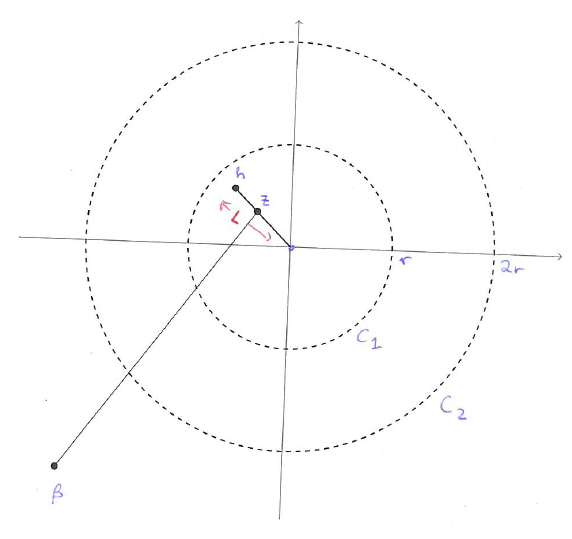
\includegraphics[scale=0.7]{ex1_q3}
\end{center}
Since $z$ lies on $L$, it is clear that $\abs{h-z} \leq \abs{h}$ (more formally, we can write $z=th$ for some $t$ with $0 \leq t \leq 1$, so that $\abs{h-z} = \abs{(1-t)h} = (1-t) \abs{h} \leq \abs{h}$).

The backwards triangle inequality, together with the fact that $\abs{z}<r<2r<\abs{\beta}$ gives
\begin{align*}
\abs{\beta - z} & \geq \abs{\abs{\beta}-\abs{z}} \\
& = \abs{\beta} - \abs{z} \\
&> 2r-r = r.
\end{align*}

Combining these two inequalities we see that
\begin{align*}
\abs{ \frac{h-z}{\beta - z} } &= \frac{\abs{h-z}}{\abs{\beta -z}} \\
 & \leq \frac{\abs{h}}{\abs{\beta - z}} \\
 & < \frac{\abs{h}}{r}.
\end{align*}

\end{answer}
\question The function $\mathbf{f}: \R^2 \to \R^2$ is defined by
$
\mathbf{f} (x,y)=(0,2y).
$
Show that the corresponding complex function $f:\C \to \C$ is
$
f(z) = z- \conj{z},
$
and that
\[
\lim_{h \to 0} \frac{f(z_0+h)-f(z_0)}{h}
\]
does not exist at any point $z_0 \in \C$.
\begin{answer}
The corresponding function is
\[
f(z) = f(x+iy) = i(2y) = i ( 2 \Im (z) ) = 2i \cdot \frac{z-\conj{z}}{2i} = z - \conj{z}.
\]
If $z_0 \in \C$ and $h \in \C \backslash \set{0}$ then
\[
\frac{f(z_0+h)-f(z_0)}{h} = \frac{(z_0+h)-\conj{(z_0+h)} - (z-\conj{z})}{h} = \frac{h-\conj{h}}{h} = 1- \frac{\conj{h}}{h}.
\]
Looking at restricted limits along the real and imaginary axes:
\[
1-\frac{\conj{h}}{h} \to \begin{cases}
1-1=0 & \text{ as } h \to 0, h \in \mathbb{R} \\
1-(-1)=2 & \text{ as } h \to 0, h \in i \R.
\end{cases}
\]
Since the restricted limits are not equal the (unrestricted) limit does not exist for any $z_0 \in \C$.

\end{answer}
\question Same as question 5 but with
\[
\mathbf{f}(x,y)=(x^2-y^2-x,2xy+y+1) \quad\text{ and }\quad f(z)=z^2-\conj{z}+i.
\]
\begin{answer}
This time, it is easier to start with the complex function $f$ and substitute $z=x+iy$:
\begin{align*}
f(z) & = z^2-\conj{z} + i \\
& = (x+iy)^2-(x-iy)+i \\
& = x^2-y^2+i2xy -x +iy +i \\
& = x^2-y^2-x + i \left( 2xy+y+1 \right),
\end{align*}
which shows that $f$ corresponds to the function $\mathbf{f}:\R^2 \to \R^2$ where
\[
\mathbf{f} (x,y) = \left( x^2-y^2-x, 2xy+y+1 \right).
\]
For $z_0 \in \C$ and $h \in \C \backslash \set{0}$ the difference quotient is
\begin{align*}
\frac{f(z_0+h)-f(z_0)}{h} & = \frac{(z_0+h)^2-\conj{(z_0+h)}+i-(z_0^2-\conj{z_0}+i )}{h} \\
& = h+2z_0-\frac{\conj{h}}{h}.
\end{align*}
Looking at some restricted limits:
\begin{align*}
\rlim{h \to 0}{h \in \R \backslash \set{0}} \frac{f(z_0+h)-f(z_0)}{h} & = 2z_0-1 \\
\rlim{h \to 0}{h \in i\R \backslash \set{0}} \frac{f(z_0+h)-f(z_0)}{h} & = 2z_0+1. \\
\end{align*}
These are not equal for any $z_0 \in \C$, so the unrestricted limit
\[
\lim_{h \to 0} \frac{f(z_0+h)-f(z_0)}{h}
\]
does not exist at any $z_0 \in \C$. 
\end{answer}
\question Let $f:\C \to \C$ be defined by $f(z) = \abs{z}^2$.  Show that $f$ is differentiable at $z=0$ and nowhere else.
\begin{answer}
Since $\abs{z}^2 = z \conj{z}$,
\begin{align*}
\frac{f(z_0+h)-f(z_0)}{h} &= \frac{(z_0+h)\conj{(z_0+h)}-z_0\conj{z_0}}{h} \\
& = \frac{z_0\conj{h}+h\conj{z_0}+h\conj{h}}{h} \\
&= z_0\frac{\conj{h}}{h} + \conj{z_0}+\conj{h} \\
& \longrightarrow
\begin{cases}
2z_0 & \text{ as }h \to 0,\ h \in \R \backslash \set{0} \\
0 & \text{ as } h \to 0, h \in i\R \backslash \set{0}.
\end{cases}
\end{align*}
For $z_0 \neq 0$, the restricted limits are not equal, hence the unrestricted limit does not exist and so $f$ is not differentiable at any point $z_0 \in \C \backslash \set{0}$.

At $z_0=0$, we have
\[
\lim_{h \to 0} \frac{f(0+h)-f(0)}{h} = \lim_{h \to 0} \conj{h} = 0,
\]
so that $f$ is differentiable at $0$ with $f'(0)=0$.
\end{answer}
\question Use the rules of differentiation to find the derivatives of the following functions:
\begin{parts}
\part $f(z) = \left( z^2+4 \right)^3$
\part $g(z) = \dfrac{z+i}{z-i}$.
\end{parts}
Find the values of $f'(i)$ and $g'(1)$.
\begin{answer}
\begin{parts}
\part Since $f$ is the composition of holomorphic functions, we can use the chain rule to find $f'(z)$:
\[
f'(z) = 3 ( z^2+4)^2(2z) = 6z(z^2+4)^2 \quad \text{ for all } z \in \C,
\]
and
\[
f'(i) = 6i (i^2+4)^2 = 6i(3)^2 = 54i.
\]
\part Since the functions $z \mapsto z\pm i$ are holomorphic on $\C$, $g$ is holomorphic on $\C \backslash \set{i}$, and the quotient rule gives
\[
g'(z) = \frac{(z-i)(1)-(z+i)(1)}{(z-i)^2} = \frac{-2i}{(z-i)^2}
\]
for all $z \in \C \backslash \set{i}$.  Hence
\[
g'(1) = \frac{-2i}{(1-i)^2} = \frac{-2i}{-2i} = 1.
\]
\end{parts}
\end{answer}

\end{questions}
